\chapter{构建增强数据集:CVQA}
\section{视觉问答数据集概述}
从LeCun的MNIST数据集\citing{lecun1998mnist}到如今各式各样的计算机视觉等人工智能任务的数据集,优质的数据集已经成为了智能系统成长的“食粮”,尤其是神经网络复兴以来,计算机视觉和自然语言处理等任务的快速迭代蜕变一直都离不开数据的收集和整理工作\citing{deng2009imagenet,lin2014microsoft,rajpurkar2016squad}。关于数据更重要还是算法更重要的争论还继续,但数据集对于智能任务的训练价值是有目共睹的,当然,前提是数据集具有足够大的容量\citing{sun2017revisiting}、规范友好数据格式、较小的数据偏见等特点。视觉问答任务是在经历了计算机视觉和自然语言处理任务成功之后的新的颇具野心的构想——让系统能同时理解多模信息,并完成信息整合与推理。自从2014年以来,多个高质量的数据集为这个人工智能领域“新生儿”的快速成长提供了坚实的保障——DAQUAR\citing{malinowski2014multi}、COCO-QA\citing{ren2015exploring}、VQA\citing{antol2015vqa}、VQA 2.0\citing{goyal2017making}、CLEVR\citing{johnson2017clevr}、VQA-CP\citing{agrawal2018don}、KB-VQA\citing{wang2015explicit}。

\textbf{DAQUAR}
DAQUAR从NYU-Depth V2中带有语义分割标注的图片基础上扩展而来\citing{malinowski2014multi}。数据集包含1449张图片,图片多为室内场景,这大大地限制了数据集的场景丰富性,是该数据集的一大劣势。数据集由训练集和测试集两部分组成,训练集中包含6794对“问题-答案”,测试集中包含5674对“问题-答案”,“问题-答案”对由算法生成或是人类志愿者提供,算法生成的“问题-答案”对根据给定的模板生成,详见图\ref{DAQUAR}。

\begin{figure}[H]
	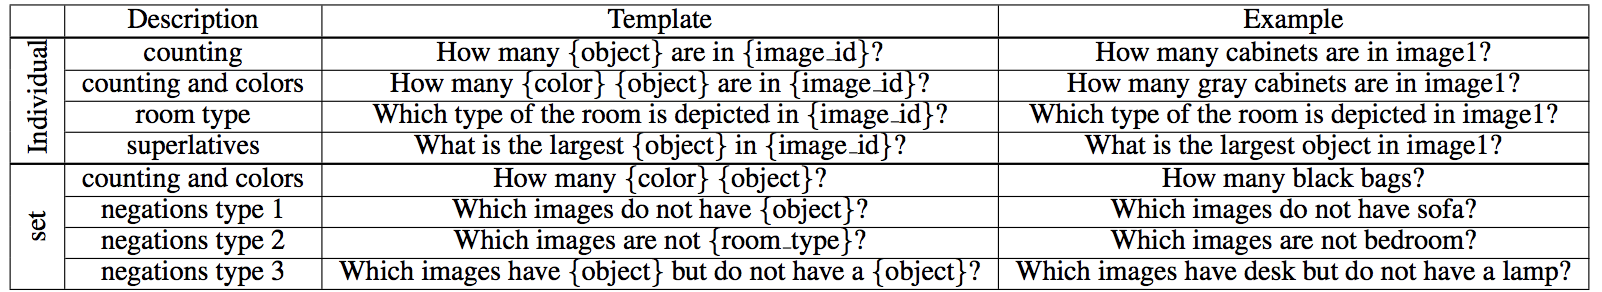
\includegraphics[width=0.8\textwidth]{DAQUAR.png}
	\caption{DAQUAR问题模板}
	\label{DAQUAR}
\end{figure}
DAQUAR数据集较小并且问题的类型只有三种:物体识别、色彩识别、计数,并且答案类型多以单词为主,因训练和测试系统复杂问题的推理能力较弱,偏于传统的物体识别任务。作为较早提出的针对视觉问答的数据集,为此后的数据集丰富工作提供了有益的方向。

\textbf{COCO-QA}
COCO-QA包含来自MS COCO的123287张真实场景图片,”问题-答案“对则是运用算法从MS COCO数据集的图片说明中生成的,为了方便生成算法的运用,将问题划分在物体识别、色彩识别、计数、地点查询四种类型。DAQUAR数据集在实际测试过程中,被发现仅仅通过简单的猜测答案的方式都能获得较高的正确率,这使得高准确率出现了极大的偏差,不能公正的测试系统的“推理”能力。为了克服该缺点,COCO-QA去除了出现频数极低和极高的一些答案,使得常见答案出现的评率从24.98\%下降到7.30\%。COCO-QA的训练集包含78736对“问题-答案”,测试集包含38948对“问题-答案”,在四个类别中的分布如图\ref{coco-vqa}。

\begin{figure}[H]
	\centering
	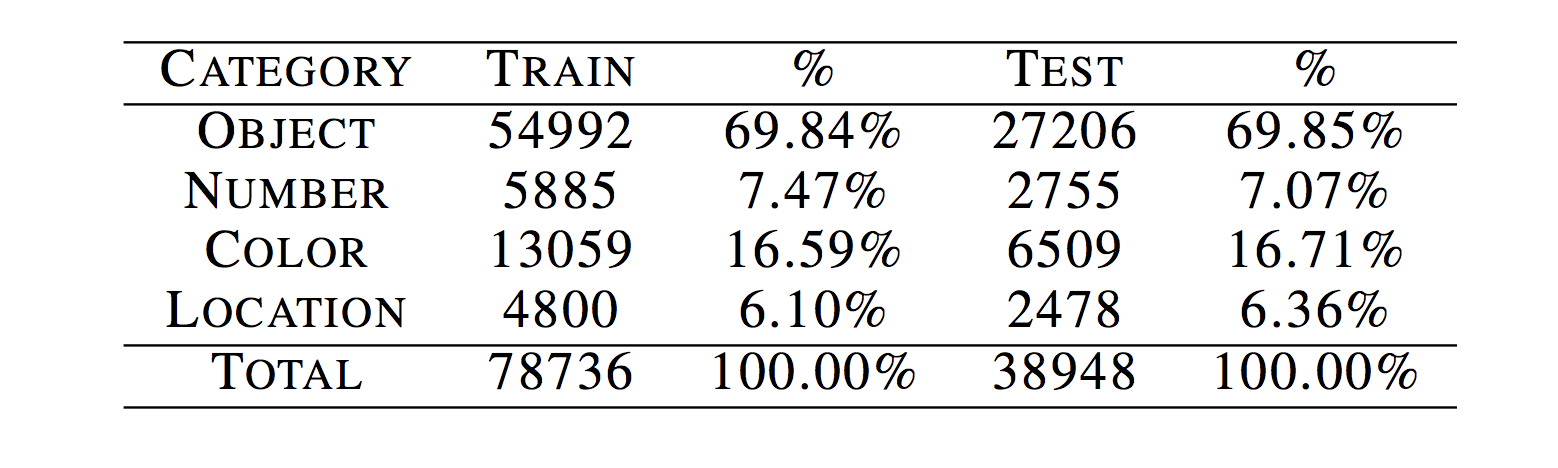
\includegraphics[width=0.8\textwidth]{coco-vqa.png}
	\caption{coco-vqa中“问题-答案”对的分布情况}
	\label{coco-vqa}
\end{figure}

\textbf{VQA}
VQA数据集是视觉问答领域发展的一个重要拐点,在此之前的数据集的问题类型被限制在一些模板之中,这使得数据集不能很好地测试出视觉问答系统在真实语境下的表现,例如,DAQUAR将答案仅仅限制在16种基本颜色和894种物体类别中\citing{malinowski2014multi}。VQA数据集中的问题和答案是无限制、开放式的,且全部由人类产生,同时图片的数量相较DAQUAR提高了两个数量级,到达254731张,极大的提高了数据集的容量。VQA数据集不仅包含从MS COCO\citing{lin2014microsoft}中提取的204721张真实场景的图片,还提供了50000张合成的抽象场景图(如图\ref{vqa-exmaple}),丰富了数据库场景的多样性,同时为高阶的场景推理和复杂空间推理提供了便利。

\begin{figure}[H]
	\centering
	\subfigure[真实场景图像实例]{
		\label{vqa-real}
		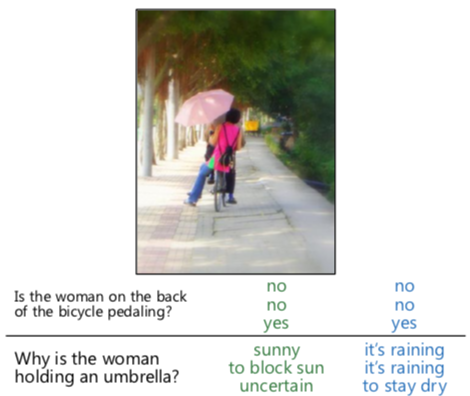
\includegraphics[width=0.4\textwidth]{VQA-real.png}}
	\subfigure[抽象场景图像实例]{
		\label{vqa-abs}
		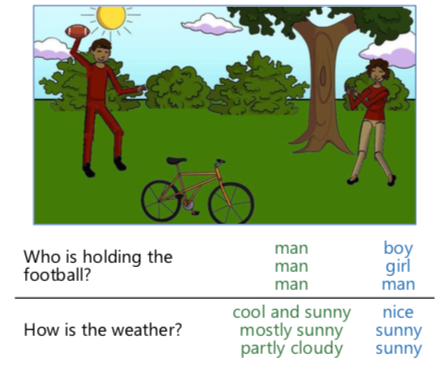
\includegraphics[width=0.4\textwidth]{VQA-abs.png}}
	\caption{VQA中的真实、抽象场景图像实例}
	\label{vqa-exmaple}
\end{figure}
为了实现对复杂推理的训练和测试,VQA数据集在问题设置上采用了人工的方式,每张图片都有3个人类提出的问题。答案则分为开放式和多项选择两种形式,开放式答案由于答案并不唯一,因此难以确定标准答案,因此正确答案的评估方法也引入人工评估机制:对于同一个开放性问题由十个人分别作答,如果有三个及以上的被测者均提供了同一答案,该答案被视为正确答案,这意味着同一个问题,可能会出现几个正确答案,这符合人类世界的真实状况,答案的不唯一性为训练智能系统多角度、多层次的“认知”提供了可能。多项选择的答案则由四种类型、18个候选项组成(如图\ref{vqa-multi}):
\begin{description}[labelindent=2em, leftmargin=6em, style=sameline]  
\item [正确答案] 一个,从被测者回答中取最为常见的作为正确答案
\item [混淆答案] 三个,不看图,仅根据问题作答的答案
\item [常见答案] 十个,数据集中最出现频数最高的十个答案
\item [随机答案] 四个,除去已经列出的选项,随机挑选四个答案
\end{description}
\begin{figure}[H]
	\centering
	\subfigure[真实场景图像的多选实例]{
		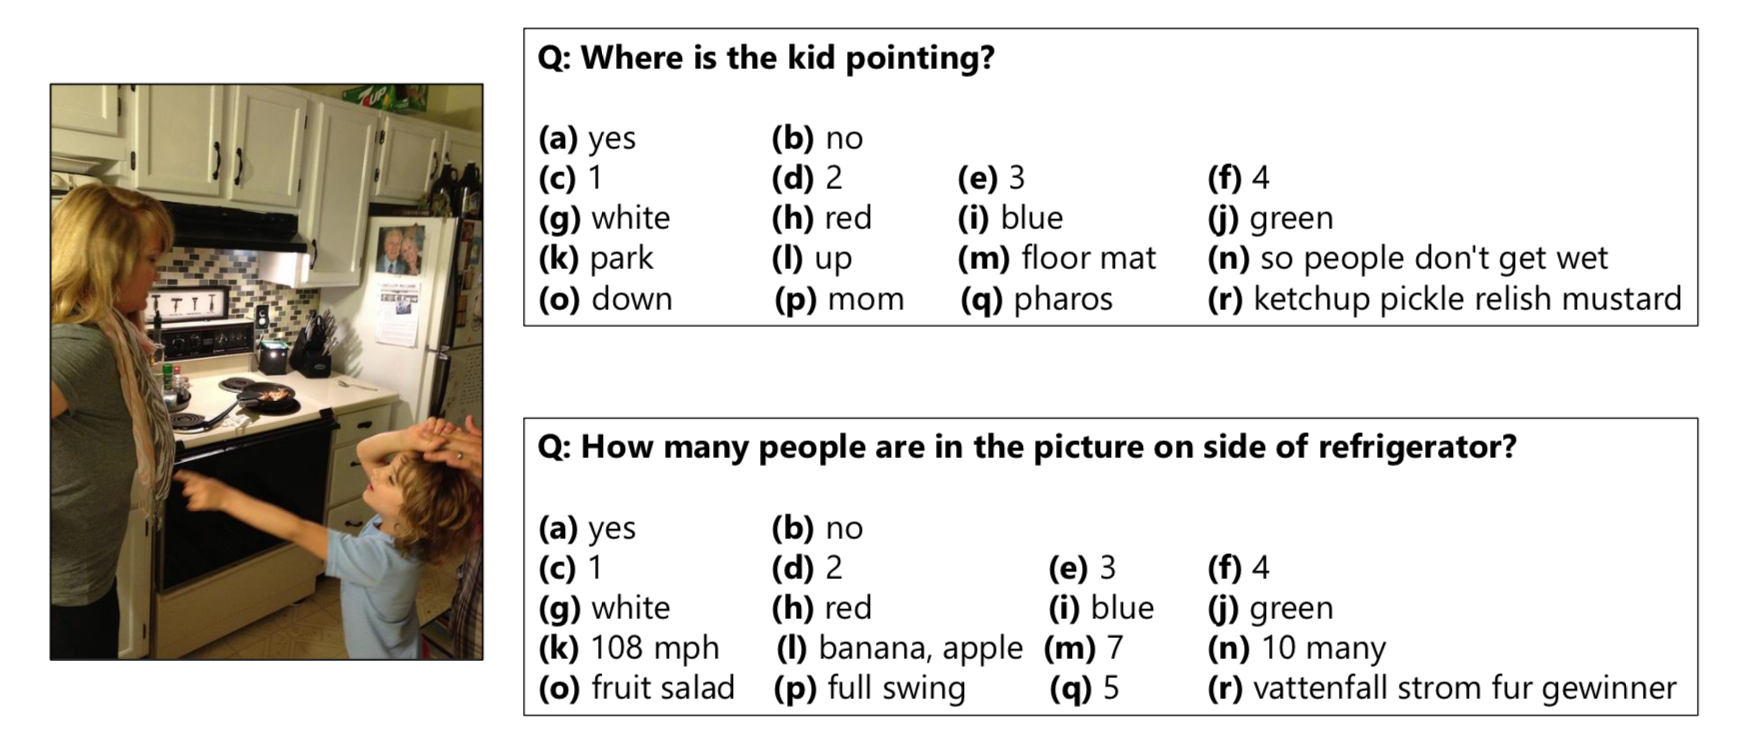
\includegraphics[width=0.8\textwidth]{vqa-multi.png}}
	\subfigure[抽象场景图像的多选实例]{
		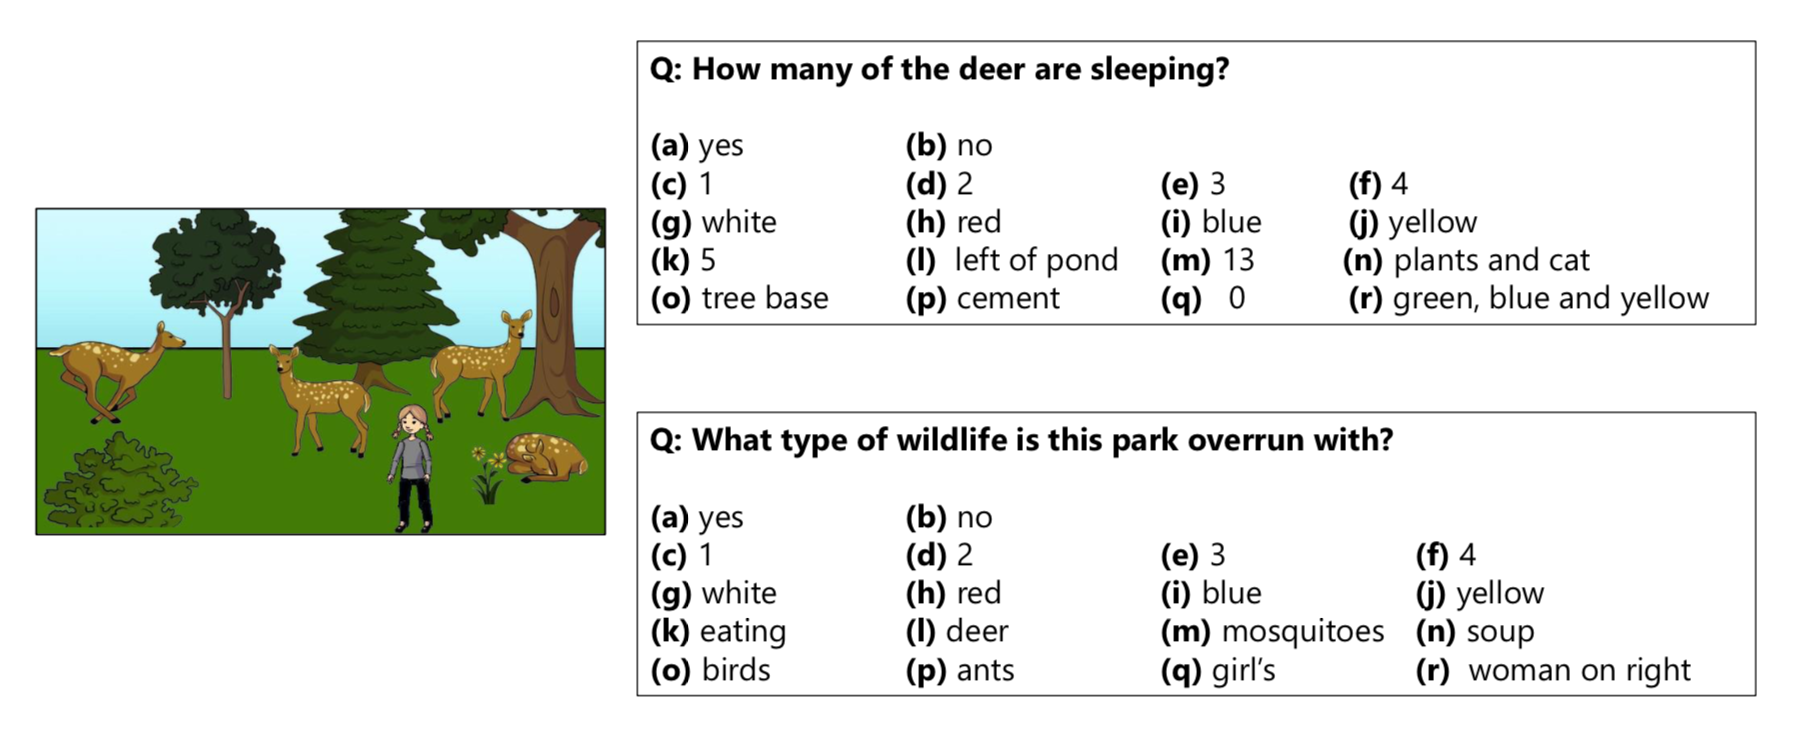
\includegraphics[width=0.8\textwidth]{vqa-multi2.png}}
	\caption{VQA中的真实和抽象场景图像的多项选择实例}
	\label{vqa-multi}
\end{figure}

\textbf{VQA 2.0}
VQA数据集由于其建立了开放性问题和多项选择问题的评测标准受到了许多研究者的追捧,成为众多算法的测试数据集,但VQA数据集中的语言偏见问题也受到了研究人员的察觉和诟病。正是由于语言偏见的问题,即使是完全无视图像的算法也能在VQA数据集上得到49.6\%的准确率\citing{ren2015exploring},这意味在VQA数据集的测试环境下,系统对于视觉信息的需求程度远远小于语言信息,这种状况相较于人类对于图像问答任务中的真实体验而言,是严重不符的。例如,答案为”是或否“的问题占所有问题的38\%,并且大约59\%的二值问题答案都为”是“;询问”什么运动“的问题中有41\%的答案为”网球;询问数量的问题中有39\%的答案为“2”。

针对以上问题,VQA 2.0应运而生。VQA 2.0通过在原有的VQA数据集基础上补充新的“混淆数据”实现数据集对视觉信息的增强。“混淆数据”和原始数据一样由(图像I,问题Q,答案A)的形式组织,不同的是新补充的图像与原有图像相似,但回答同样的问题Q却得到不同的答案A(如图\ref{vqa2})。针对同样的问题,在不同图片背景下需要得到不同的答案,这要求系统不仅能理解自然语言问题,同样需要关注图片的语义差异,才能得到正确的答案,这种平衡的方法能够筛选掉弱化图像理解的算法,强化了图像理解在视觉问答任务的重要性。补充后的VQA 2.0包含110万对”图像-问题“、20万张关联1300百万个问题的真实场景图片,数据量几乎是VQA数据集的两倍,势必会取代VQA数据集成为开放性问题的新测试标准。
\begin{figure}[H]
	\centering
	\subfigure[]{
		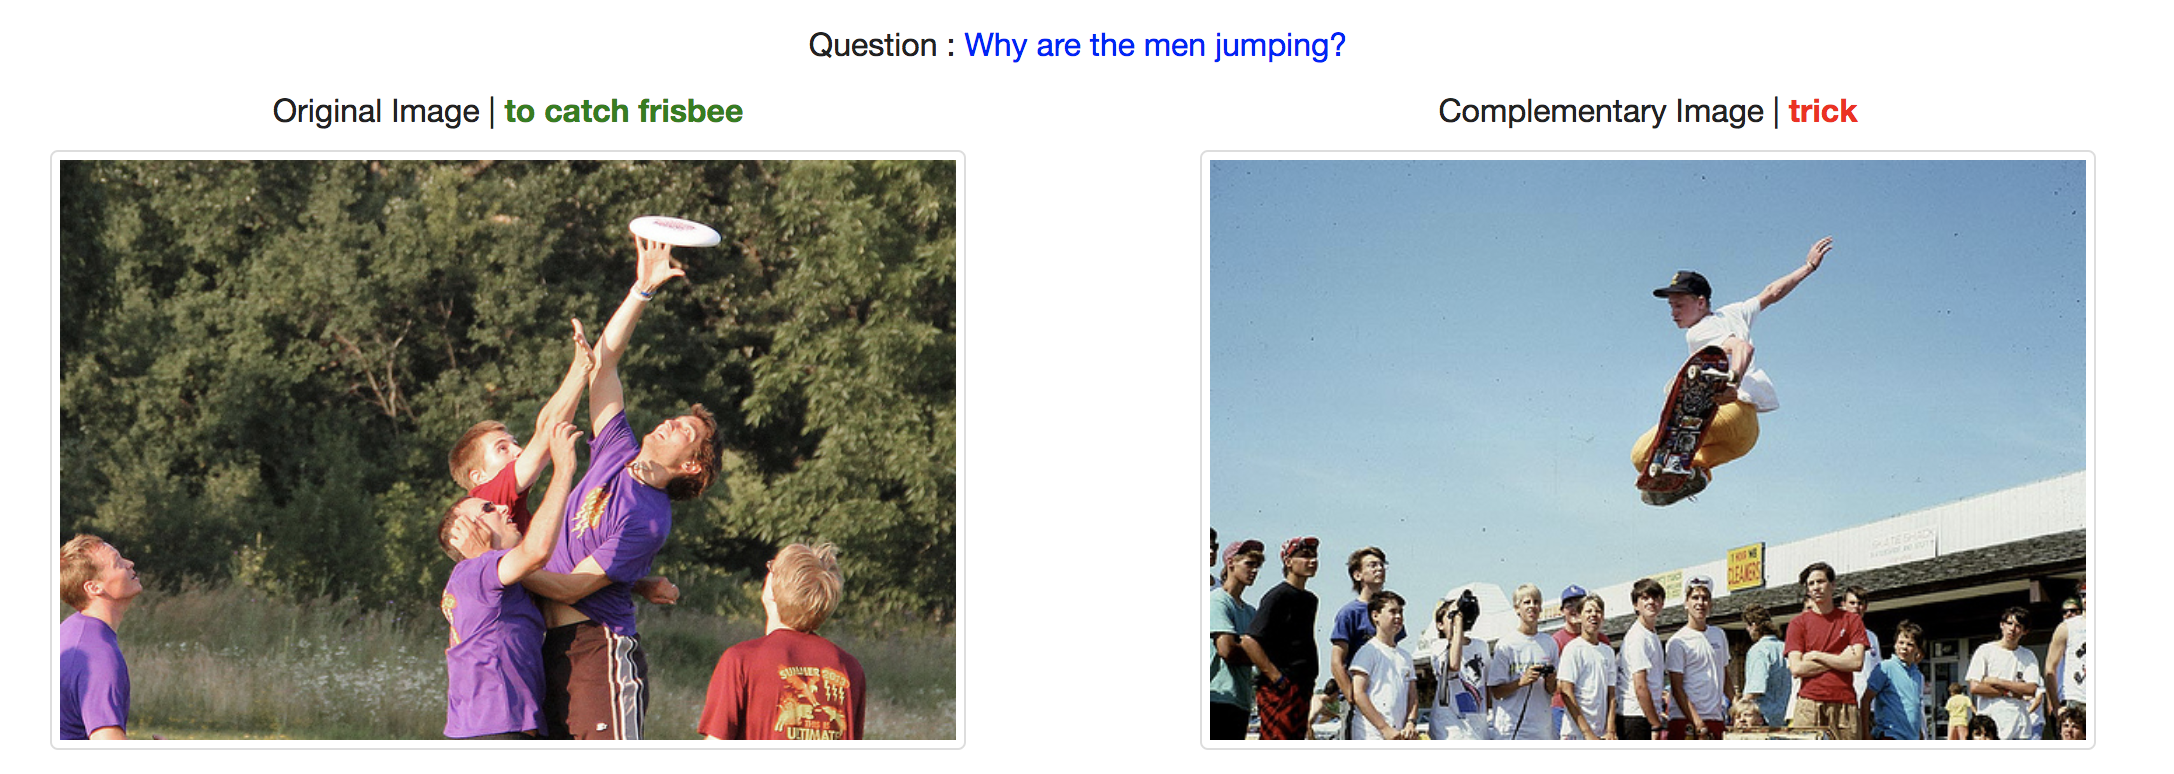
\includegraphics[width=0.8\textwidth]{vqa2-1.png}}
	\subfigure[]{
		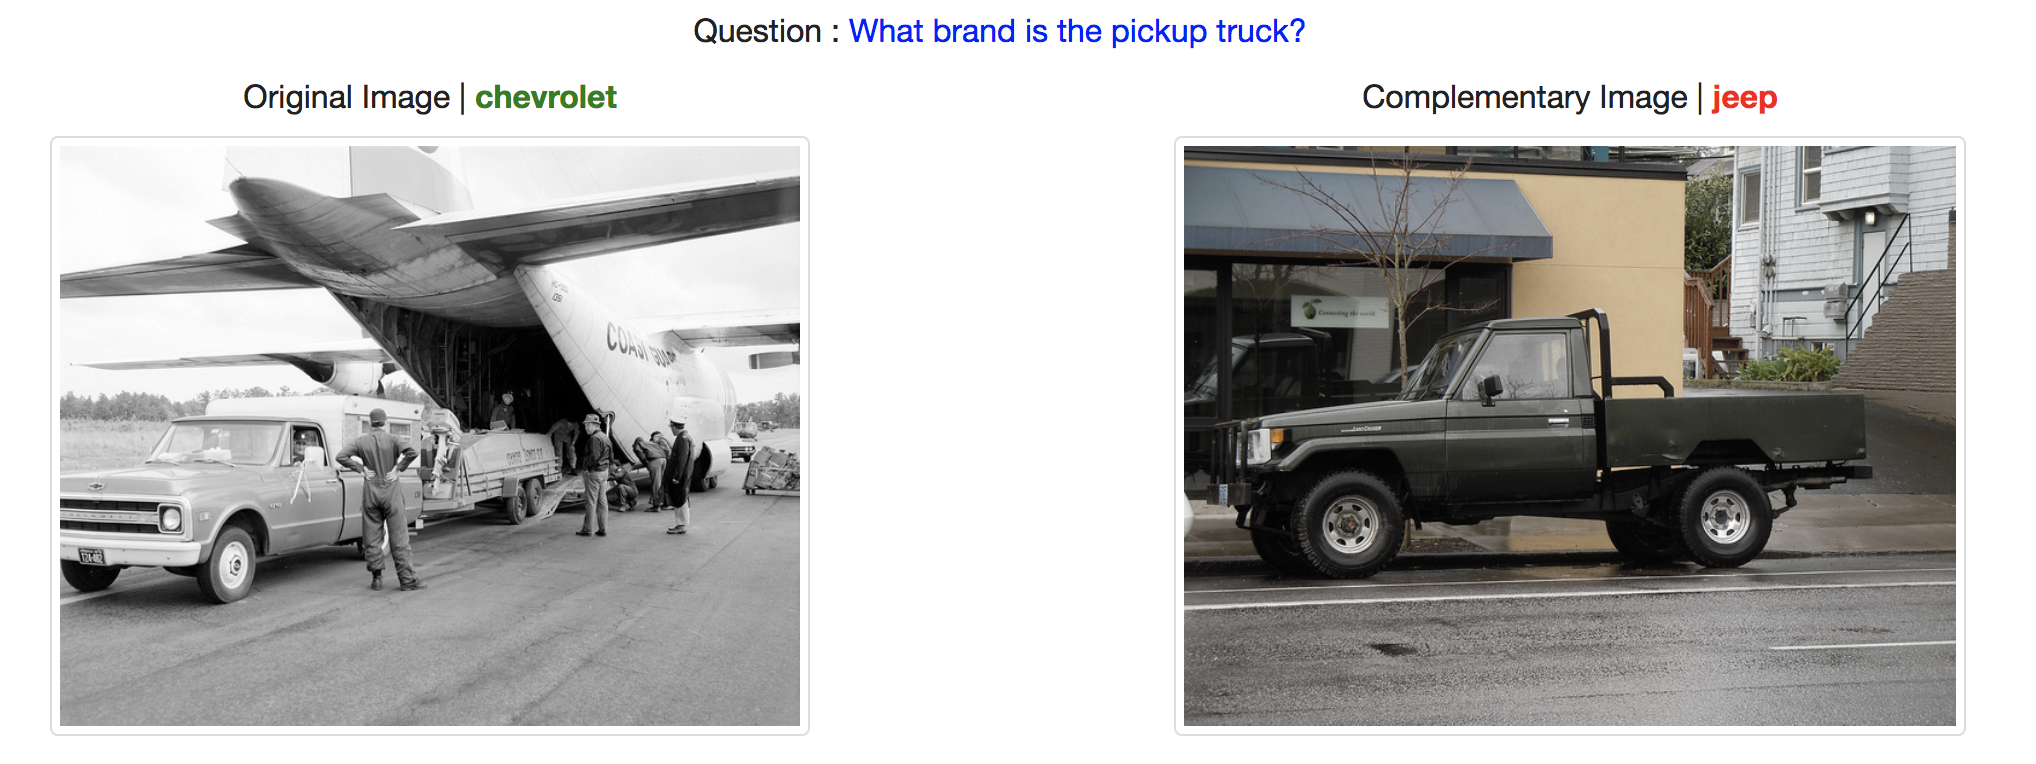
\includegraphics[width=0.8\textwidth]{vqa2-2.png}}
	\caption{VQA 2.0中针对同一问题的不同图像和答案实例}
	\label{vqa2}
\end{figure}

\textbf{CLEVR}
为了更加准确地衡量视觉问答系统各个方面的推理能力,Johnson等人提出了一个结合语言和基本视觉推理诊断数据集CLEVR。CLEVR包含10万张由空间立方体组成的合成图像、将近100万个问题,其中包含85.3万个独特的问题。在图像的设置上,CLEVR为了减小识别难度,关注系统的视觉推理能力,采用了由空间立方体组成的合成图像,并且每张图像均有包含所有物体位置和属性的说明(如图\ref{clevr})。CLEVR的问题也均由程序生成得到,涉及属性识别、计数、比较、逻辑运算等子任务。

为了减少问题的偏见,数据集生成的问题中有85\%是独特的;为了控制问题的准确性,数据集剔除了有歧义的问题,例如,询问“正方体右边的球体是什么颜色?”时,如果“正方体”右边有多个“球体”,问题便产生歧义,答案变得不唯一,使得评估过程变得复杂和不准确;为了保持问题的复杂性,数据集拒绝了一些看似复杂但实际上限定条件无效的问题,例如,询问“球体前面的圆柱体是否为金属的?”时,如果场景中仅有一个“圆柱体”,那么问题中的“球体前面”的限定便可以被忽略,这种情况降低了问题的复杂性。

由于CLEVR数据集对图像和问题具有完全的掌控,能实现其他数据集难以实现的能力测试,要求系统具有短期的记忆力、注意力机制、组合推理能力。
但同样因为其简单的图像场景设置,CLEVR不能测试出视觉问答系统在常识推理、复杂推理的表现,并且也不能衡量系统在真实场景中的识别能力和稳定性。
\begin{figure}[H]
	\centering
	\subfigure[尺寸、形状、样色、材质的标注]{
		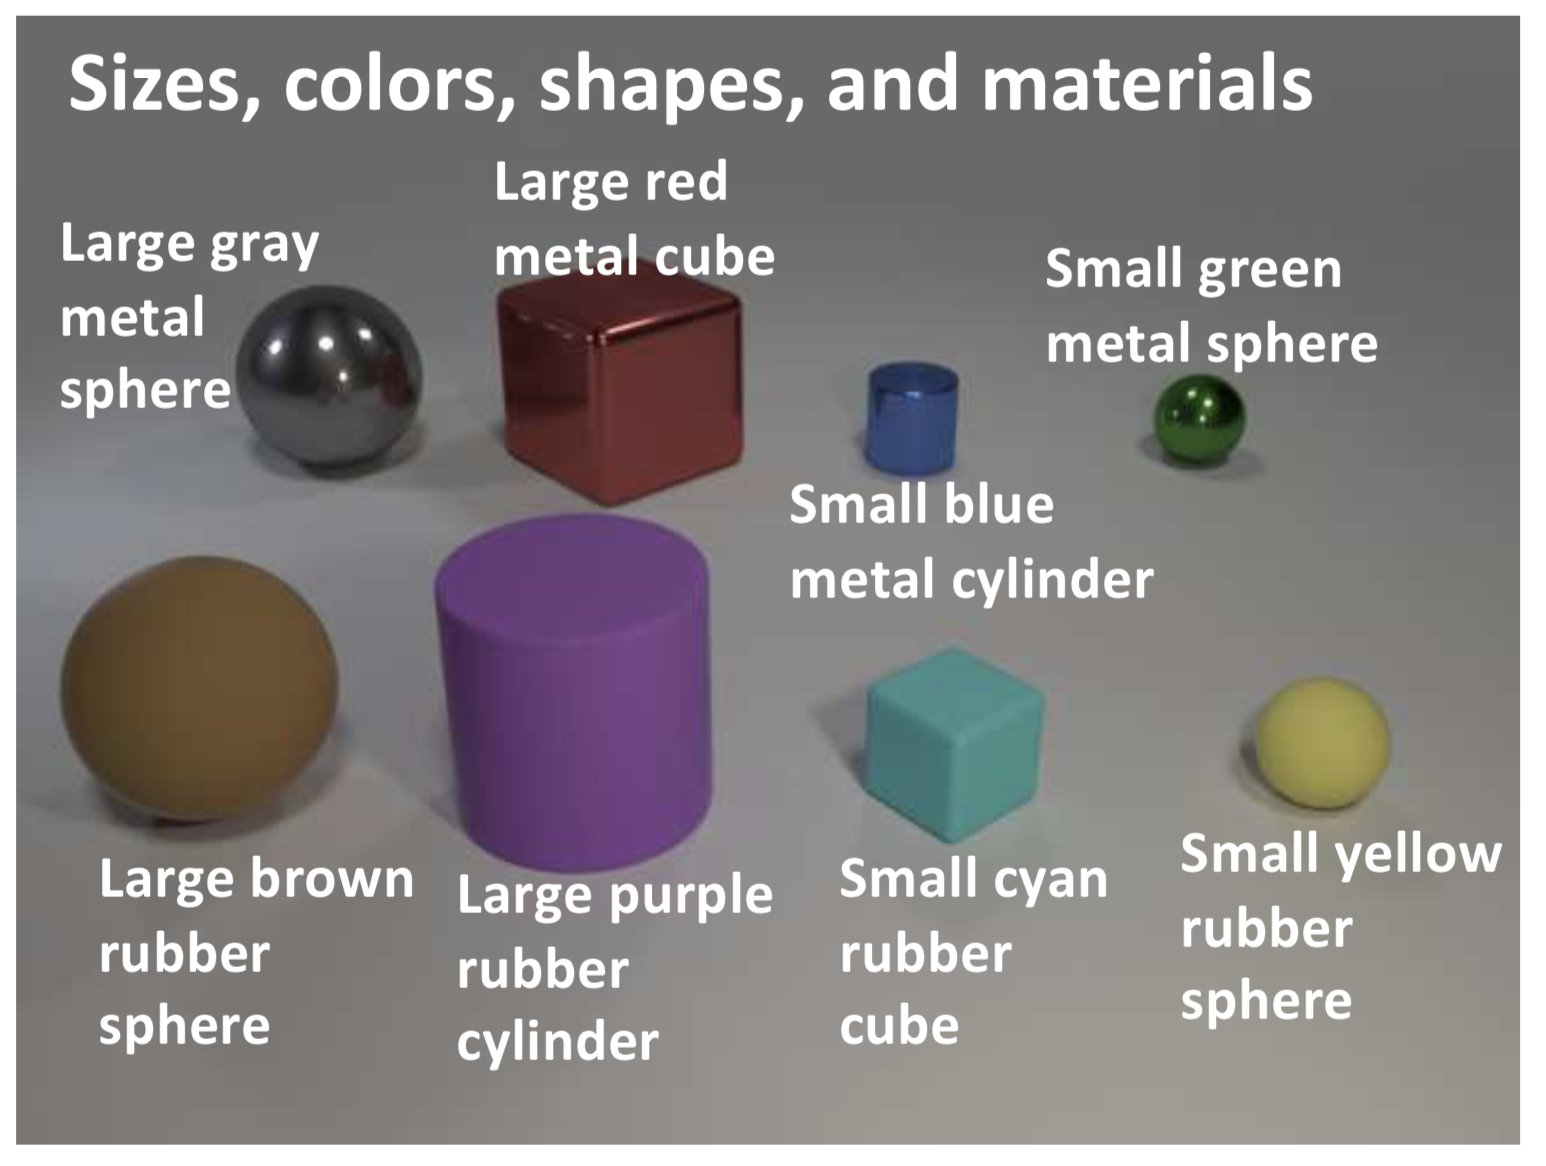
\includegraphics[width=0.3\textwidth]{clevr1.png}}
	\subfigure[空间左右的标注]{
		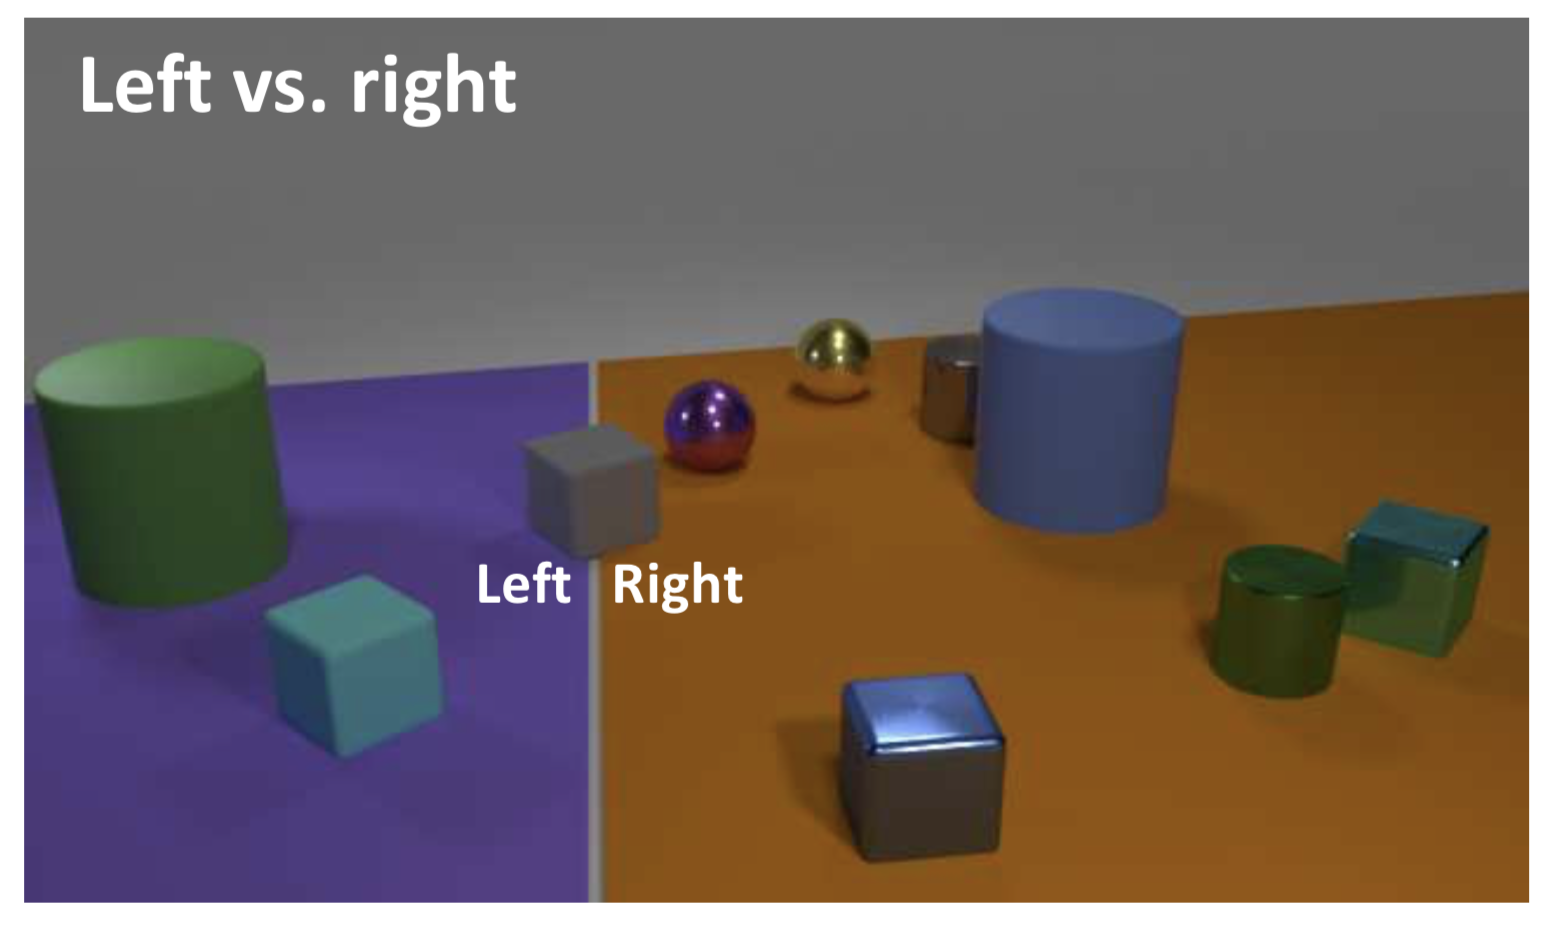
\includegraphics[width=0.3\textwidth]{clevr2.png}}
	\subfigure[空间前后的标注]{
		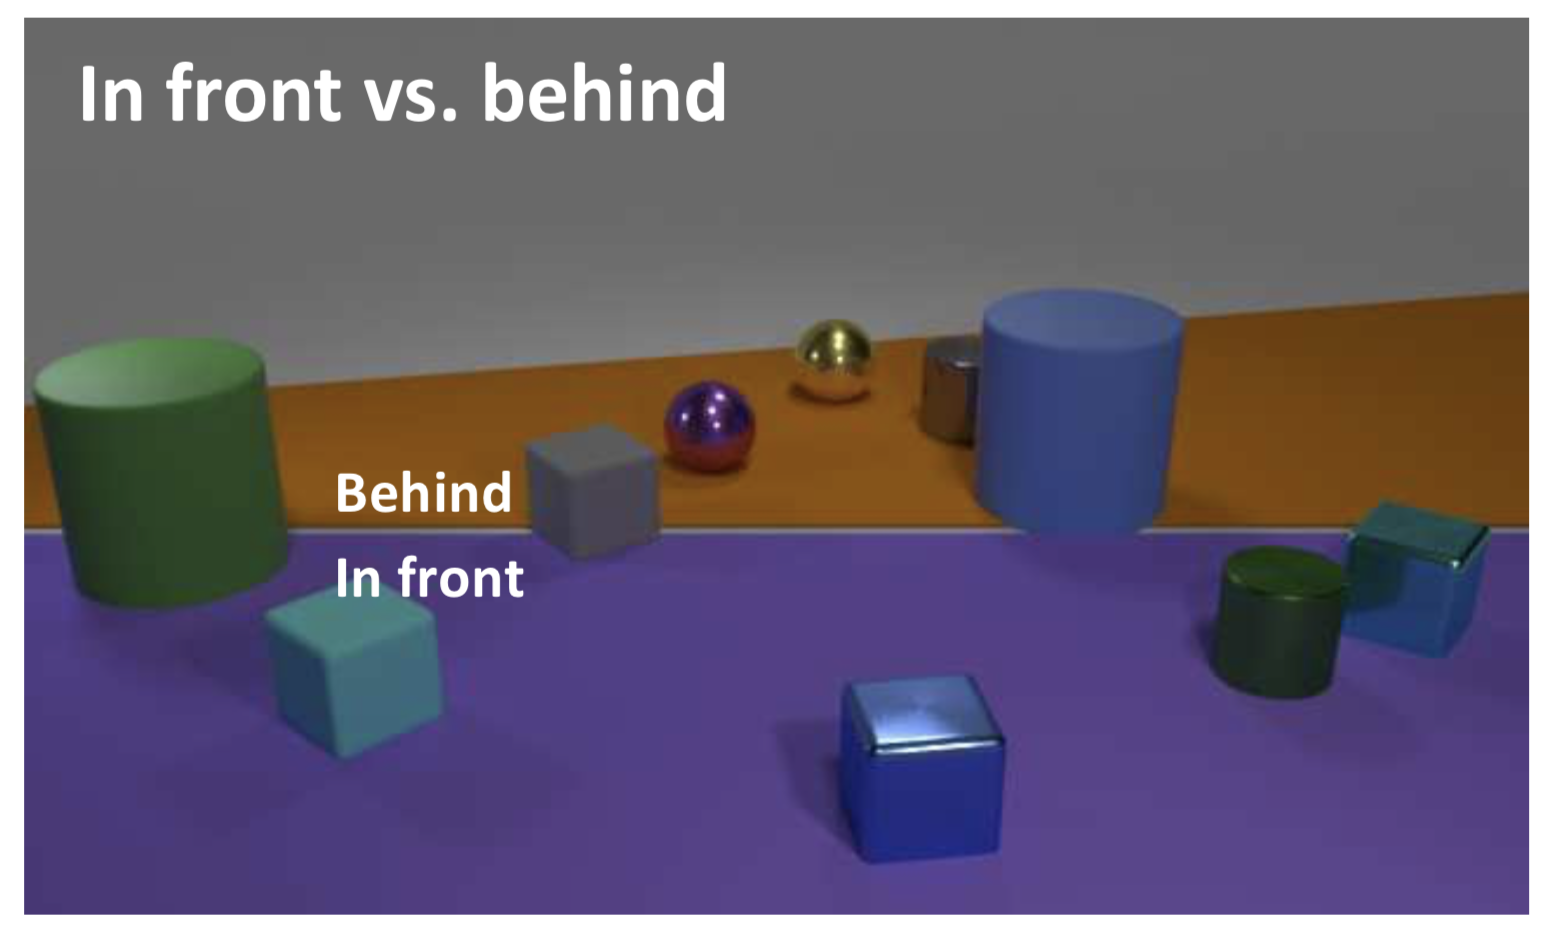
\includegraphics[width=0.3\textwidth]{clevr3.png}}
	\caption{CLEVR中图像标注}
	\label{clevr}
\end{figure}

\textbf{VQA-CP}
数据集一般会划分为训练集和测试集两个部分,在视觉问答任务中同样如此。如果训练集中的答案分布存在偏见,且测试集与训练集之间的答案分布相近,那么系统便可以通过记忆在训练过程中得到的数据偏见,并将其应用于测试过程,这样得到的准确率的可信度将会打折扣,例如,在训练集中询问颜色的问题中“白色”最为常见,同样在测试集中的“白色”也为热门答案,这回干扰系统的评估结果,不清楚系统是通过正确推理得到还是”经验“得到的。

针对训练集和测试集中问题答案分布相似的状况,VQA-CP重新对VQA数据集和VQA 2.0进行划分,重新划分得到的训练集和测试集在每个问题类型中的答案分布均不同,例如,在训练集中询问颜色的问题中,“白色”、“红色”为最常见的答案,而在测试集中“黑色”、“粉色”为最常见的答案;对于询问运动类型的问题,在训练集中“网球”为最多的答案,而在测试集中“滑雪”为最常见的答案(如图\ref{vqa-cp})。
\begin{figure}[H]
	\centering
	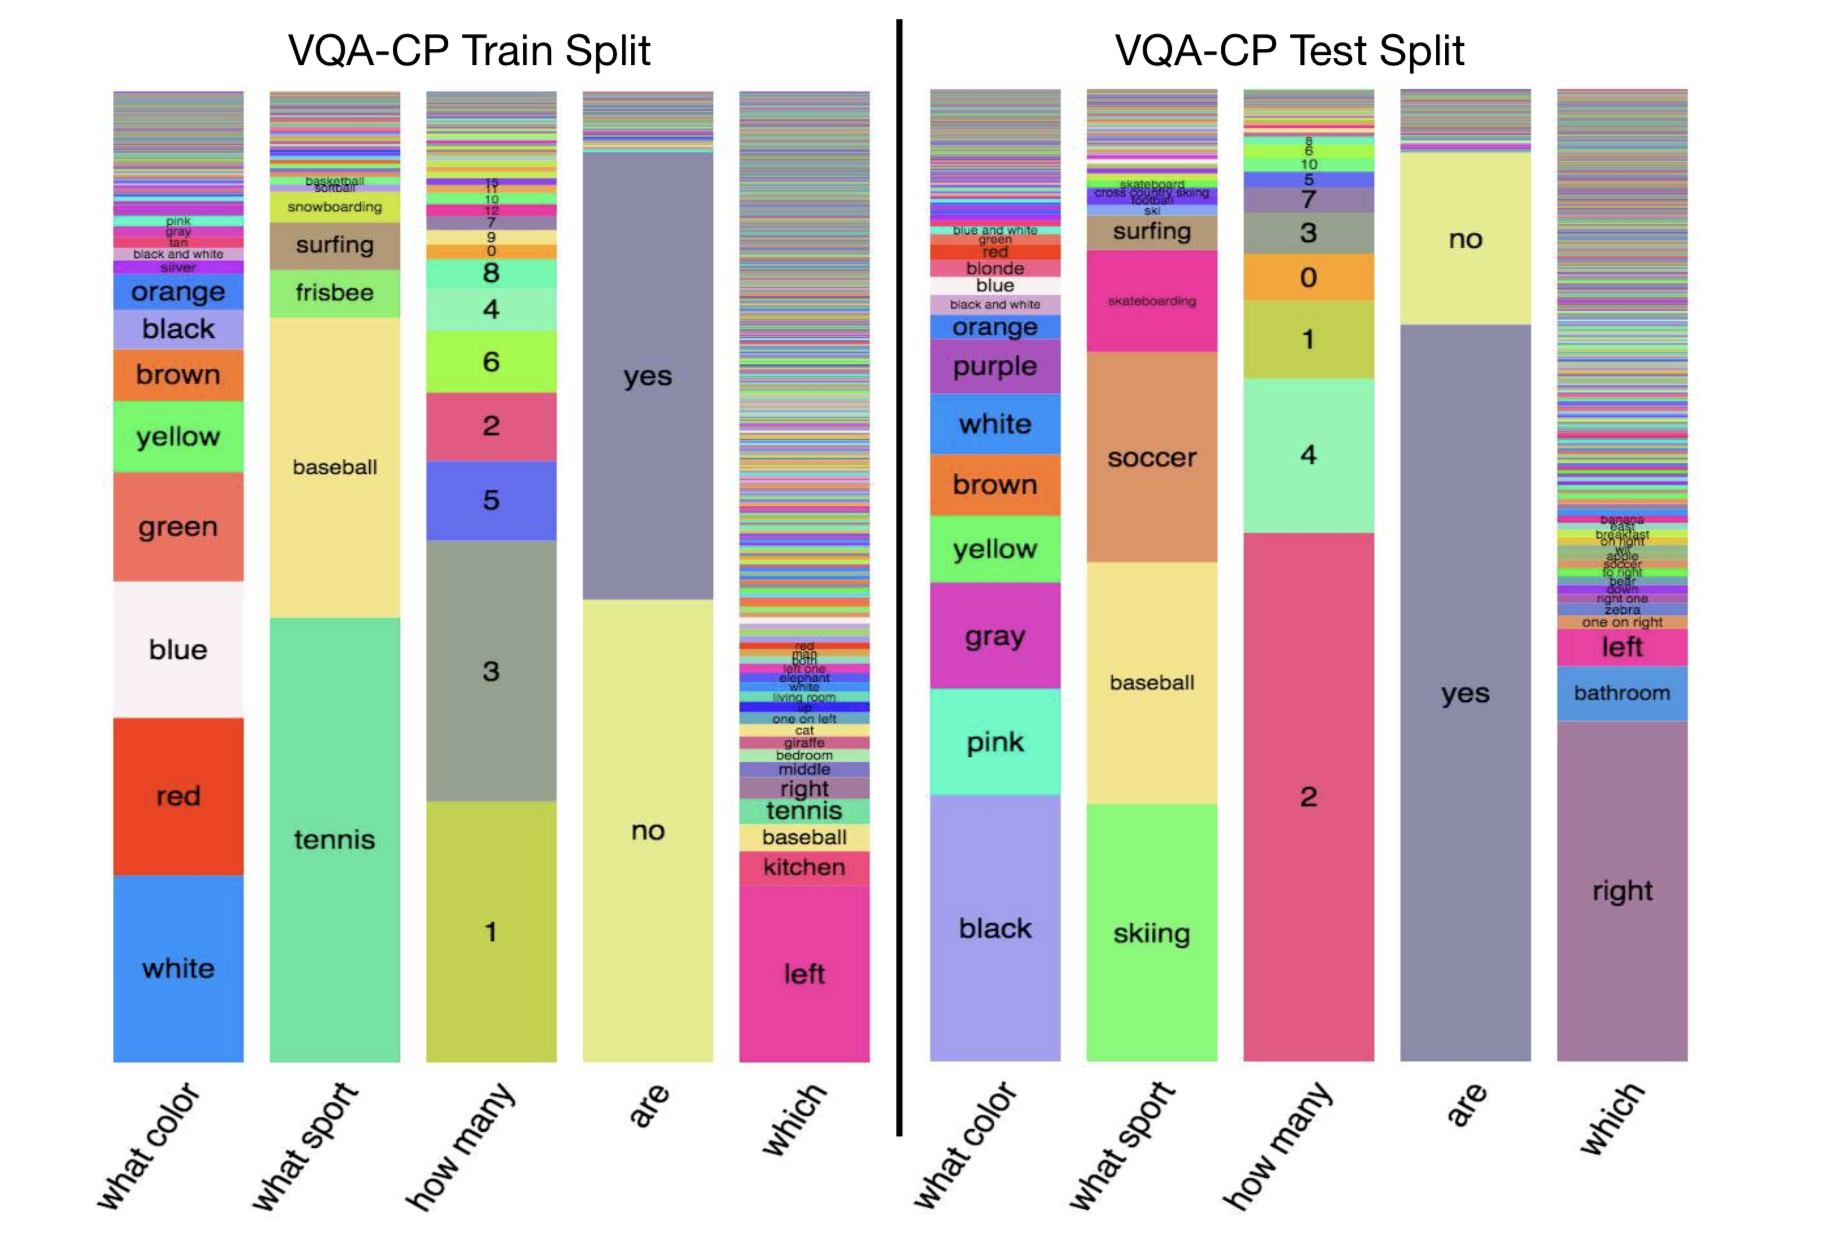
\includegraphics[width=5in]{vqa-cp.png}
	\caption{vqa-cp训练集和测试集的答案分布}
	\label{vqa-cp}
\end{figure}

\textbf{KB-VQA}
回答VQA等数据集中的开放性问题可能涉及常识或者特定领域知识的先验知识,但已有数据集中还掺杂着大量不需要先验知识的训练样本,因此为了更好的评估VQA算法对需要高层次知识问题的准确推理能力,Wang等人构建了只包含复杂推理问题的数据集KB-VQA\citing{wang2015explicit}。

KB-VQA数据集从MS COCO\citing{lin2014microsoft}中挑选出700张图片样本,挑选出的图片包含150个物体类别和100个场景类别。每张图片附带有3-5个由人工生成的“问题-答案”对,所有的问题被限定在23种问题模板中,例如,“图片中是否存在某种概念?”,“图片中的某个物体被生产于什么地方?”等,详见\ref{qt}。

为了准确评估系统在需要先验知识的问题的表现,KB-VQA人工地赋予每个问题一个表示所需不同知识类型的标签,“视觉问题”、“常识问题”和“知识库问题”,其中“视觉问题”表示仅仅从图片中便可以获得答案的问题,例如,“物体是否存在于图片?”、“列出图片中包含的所有事物?”等,“常识问题”需要结合成人级别的常识和图像内容得出答案,例如,“图片涉及什么场景?”,“知识库问题”则需要某个领域特定的知识才能完成作答,例如,“图中的物品在哪一年被发明?”。23种问题模板在不同问题标签的分布如图\ref{qtd}。
\begin{figure}[H]
	\centering
	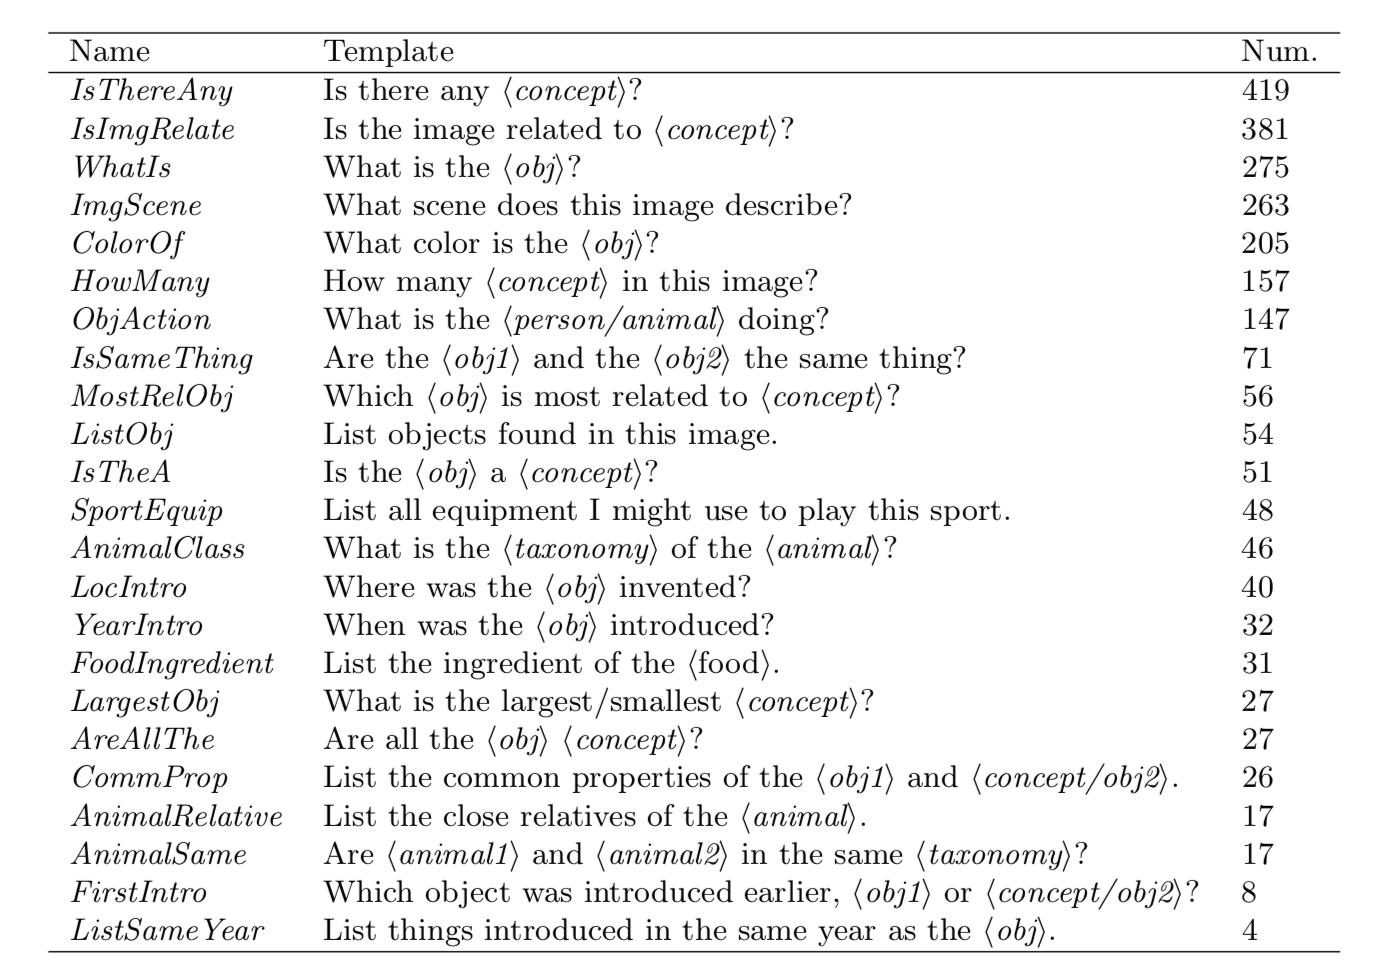
\includegraphics[width=0.8\textwidth]{qt.png}
	\caption{KB-VQA中23中问题模板及对应的问题数量}
	\label{qt}
\end{figure}
\begin{figure}[H]
	\centering
	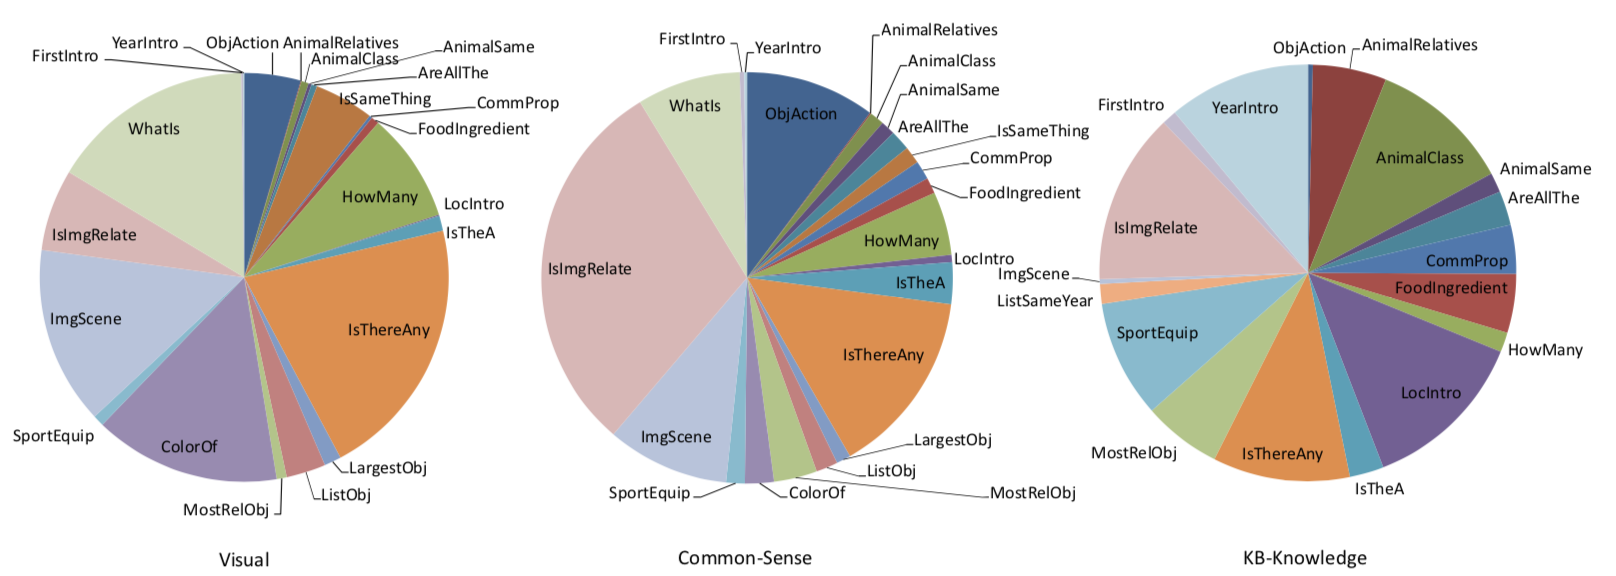
\includegraphics[width=0.8\textwidth]{qtd.png}
	\caption{KB-VQA中23中问题模板对应“视觉问题”、“常识问题”和“知识库问题”的分布情况}
	\label{qtd}
\end{figure}

数据集中的“视觉问题”、“常识问题”和“知识库问题”数量分别是1256、883和263,就图片和问题的数量而言,KB-VQA数据集相较于COCO-QA等数据集是非常小的,而且从图\ref{qt}也容易看出,有16种问题类型的问题数量都不超过100个,甚至有个位数的问题数量,数据集的不均衡和小容量很难准确得评估出系统在细分问题类型上的推理能力。但需要先验知识的问题占比要远高于大型数据集,DAQUAR\citing{malinowski2014multi}几乎全是“视觉问题”,COCO-VQA\citing{ren2015exploring}仅仅包含5.5\%的问题需要常识,没有问题需要额外的知识库。

KB-VQA在评估系统的复杂推理能力方面提供了一个解决方案,但数据集的容量、平衡性和多样性方面还需要更多的丰富,并且随着数据集的扩充,自动化和标准化的评估方式也相应的需要完善。

\textbf{FVQA}
为了评估视觉问答系统在需要先验知识的问题上的表现,Wang等人提出了FVQA数据集\citing{wang2017fvqa}。回答FVQA中的问题需要额外的知识,但不同于一般的数据集,FVQA将(图片,问题,答案)的三元组数据扩展为(图片,问题,答案,支持事实)的四元组形式,其中“支持事实”是回答问题所需要的额外知识,使用资源描述框架(RDF)的三元组形式,例如(猫,可以,爬树)。

FVQA从MS COCO\citing{lin2014microsoft}和ImageNet\citing{deng2009imagenet}中挑选出1906张图片,并对图片预处理,提取出三种类型的视觉概念:物体对象、场景和行为,最终提取出326种物体对象、21种场景和24种行为。为了获取与视觉概念相关的知识,FVQA以DBpedia\citing{auer2007dbpedia}、ConceptNet\citing{liu2004conceptnet}和WebChild\citing{tandon2014webchild}为知识源,从三种知识库中与视觉概念相关的所有知识中筛选出包含12种常见的谓语的知识,例如,关于分类的知识——“目录属于”、关于地点的知识——“地点所在”、关于大小比较的知识——“体积大于”,详见图\ref{fvqa_vc}。提取的知识以资源描述框架(RDF)的形式存储作为“支持事实”。
\begin{figure}[H]
	\centering
	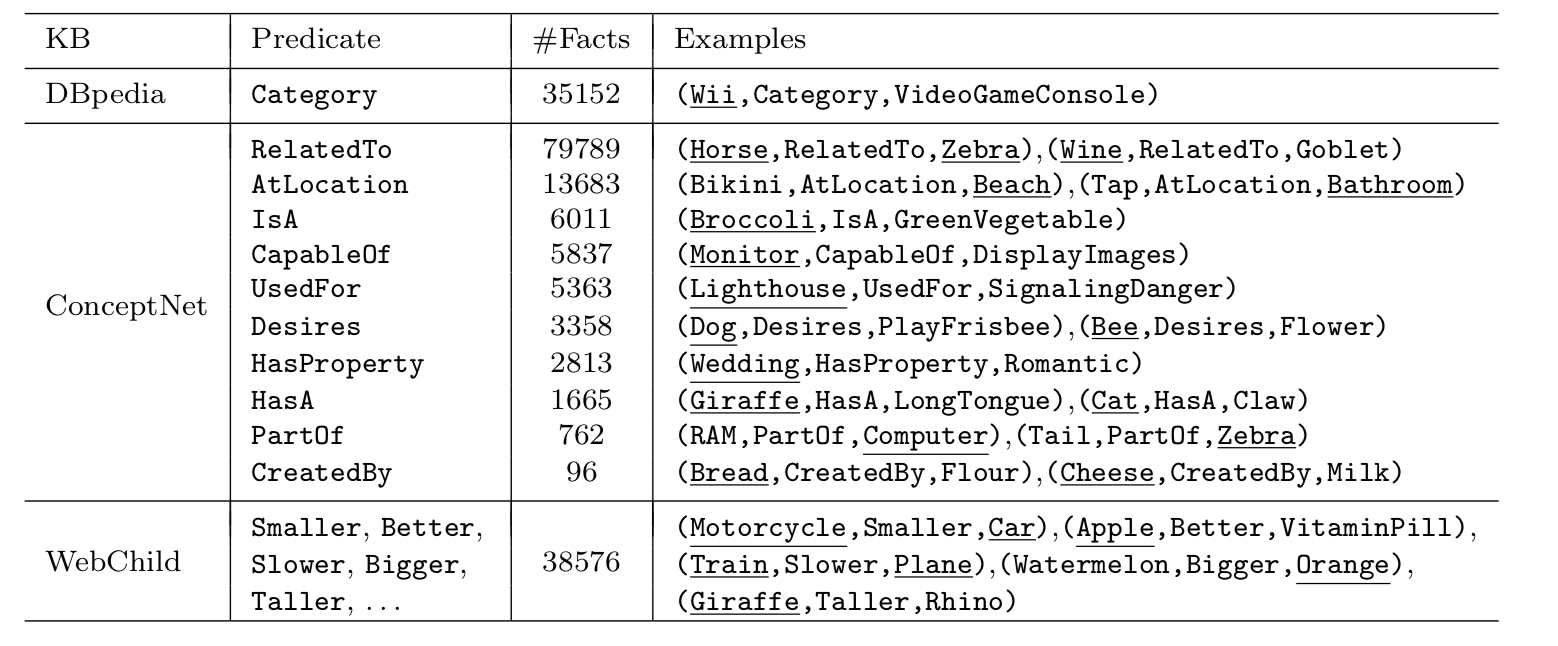
\includegraphics[width=0.8\textwidth]{fvqa_vc.png}
	\caption{从三种知识库中提取的知识涉及的12种谓语及相应的数量}
	\label{fvqa_vc}
\end{figure}

FVQA的问题和答案均使用人工的方式收集得到,被试者先选择图片中的一个视觉概念和一个与视觉概念相关的支持事实,再根据视觉概念和支持事实给出问题和答案,答案的来源要么是图片中的视觉概念要么是支持事实中涉及的概念。数据集最终包含4608个需要先验知识的问题,涉及3458条事实。根据视觉概念的类型,这些问题可以归为物体对象、场景和行为三种类型;根据支持事实的来源,可以归为DBpedia、ConceptNet和WebChild三种类型;根据答案来源,可以归为图片来源和知识库来源两种类型,不同分类在训练集和测试集的数量分布如图\ref{fvqa_cd}。
\begin{figure}[H]
	\centering
	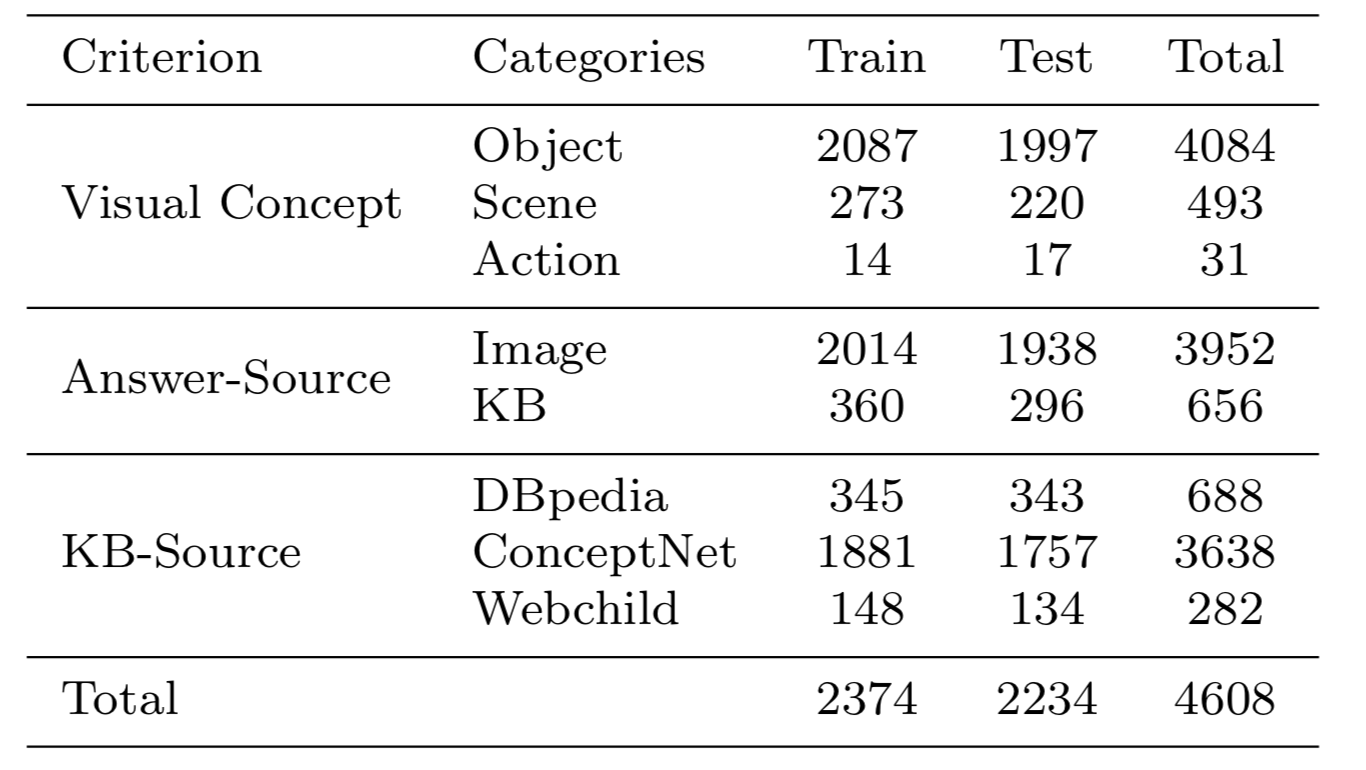
\includegraphics[width=0.8\textwidth]{fvqa_cd.png}
	\caption{不同分类在训练集和测试集的数量分布}
	\label{fvqa_cd}
\end{figure}

从统计的数据上不难看出,绝大多数问题是针对图像中的物体对象,这与提供的视觉概念中物体对象的高占比有强关联,从知识来源上分析,答案除了能从图像中获得外,还包含14\%的答案需要从额外知识库中获得,并且问题中不包含“是或否”的二值问题,这降低了系统”猜中正确答案“的情况。

FVQA和同样包含先验知识的数据集KB-VQA两者都能通过查询语言获取知识库中的数据,但不同于KB-VQA,FVQA拥更多的图片和问题数量,并且所有问题都需要额外知识。FVQA增加了ConceptNet和WebChild作为知识源,提高了知识库的多样性,能回答更多类型的问题,而不用预先设定问题模板。但FVQA数据集中几乎所有的答案都是物体对象,且为单个词语,不能训练模型给出对象关系的答案。FVQA数据集的支持事实多为单一谓语的句子,句式结构简单,如果用做训练集,不能考察模型应对多动词结构问题时的答案正确率。

然而两个数据集都面临着同样的问题:数据量的扩充和问题类型的扩充。两个数据集的问题收集都是通过人工的方式,并且参与者数量有限,因此直接导致了问题数量远低于其他自动化方法生成的数据集。大规模的协同工作和探索更多自动化方法是扩充数据集容量的方向。两个数据集都受到问题类型的限制,KB-VQA使用预先设定的问题模板,限制了问题的开放程度,FVQA虽然没有使用预先设定的问题模板,但其筛选的12种谓语间接的限制了问题的类型。扩展问题类型意味着额外知识库的扩充,也对视觉问答系统的问题解析提出了更高的要求,但这也能大幅的提高系统面对复杂多样的问题的开放性和鲁棒性。

\section{CVQA的构建和分析}

